\chapter{Oprogramowanie}
\label{ch:soft}

\section{System operacyjny}
Najczęściej używanym systemem operacyjnym na platformie Raspberry Pi jest Raspbian. Jest to
darmowa dystrybucja Linuxa oparta na Debianie, odpowiednio dostosowana do pracy z Respberry Pi. System jest udostępniony przez twórców na stronie organizacji \cite{raspfoundation} Raspberry Pi Foundation zarówno w wersji 'Raspbian with Desktop' ze środowiskiem graficznym PIXEL (z ang. Pi Improved Xwindows Environment, Lightweight), jak i w wersji bez środowiska graficznego Raspbian Lite.

Raspbian jest wielozadaniowym systemem operacyjnym, więc przydziela wszystkim programom czas procesora według algorytmu szeregowania. Z punktu widzenia aplikacji użytkownika nie wiadomo kiedy nastąpi wywłaszczenie i na jak długo. Jest to problematyczne w przypadku obsługi krytycznych czasowo zadań.
Rozwiązaniem może być zastosowanie modułu do jądra systemu operacyjnego i wykonanie krytycznych czasowo zadań w funkcji obsługi przerwania lub uruchomienie aplikacji na systemie czasu rzeczywistego (z ang. RTOS - Real Time Operating System) takim jak FreeRTOS lub ChibiOS. Systemy operacyjne czasu rzeczywistego zawierają mechanizmy ułatwiające implementacje systemu akwizycji danych. 
Podczas kompilacji jądra Linuxa istnieje możliwość dodania rozszerzeń czasu rzeczywistego, które udostępniają funkcje w przestrzeni jądra i użytkownika, ułatwiające implementację krytycznych czasowo aplikacji w systemie.

\section{Środowisko Buildroot}

Buildroot jest narzędziem umożliwiającym użytkownikowi stworzenie okrojonej na potrzeby danego zastosowania wersji systemu wbudowanego Linux. Środowisko to składa się z zestawu plików Makefile i kconfig, które upraszczają przygotowanie cross-kompilacji za pomocą zestawu narzędzi \ang{toolchain} dla danej architektury. Producent dostarcza również domyślne konfiguracje do kilku popularnych platform m.in. Cubieboard i Raspberry Pi, co skraca czas rozpoczęcia projektu systemu. W pobranym ze strony producenta pliku w katalogu \ang{board} (Rys. \ref{fig:brakat}) znajduje się katalog raspberrypi zawierający domyślną konfigurację dla platformy Raspberry Pi 3.
\begin{figure}[h]
	\centering
		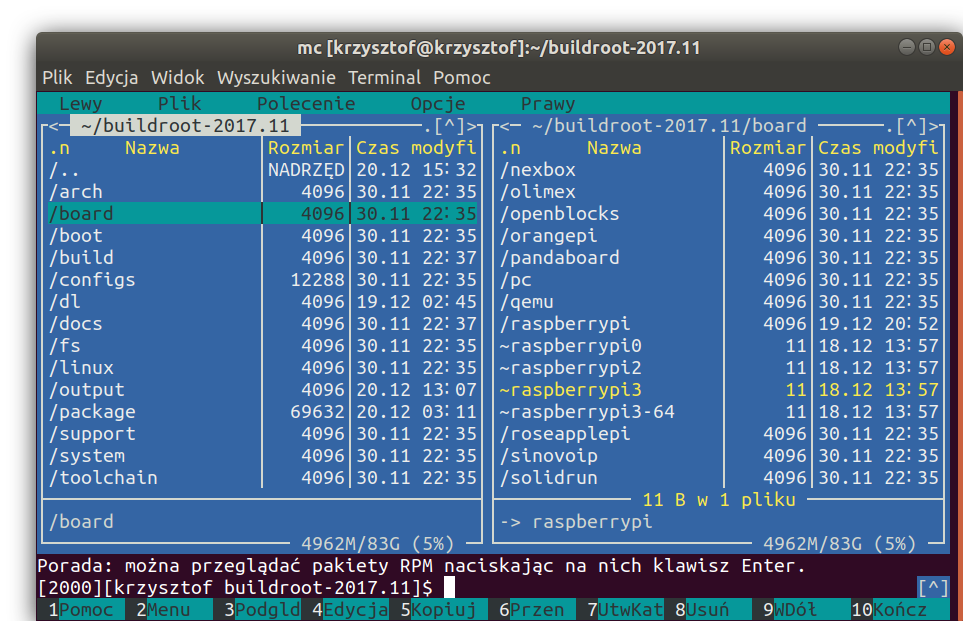
\includegraphics[width=13cm]{buildroot_katalogi}
	\caption{Katalog board z plikami konfiguracyjnymi} 
	\label{fig:brakat}
\end{figure}

Buildroot pozwala ustawić opcję dwóch rozszerzeń czasu rzeczywistego XENOMAI i RTAI. Są to rozszerzenia wykorzystywane w systemach wbudowanych do wspierania aplikacji czasu rzeczywistego.
RTAI (z ang. real time application interface - interfejs dla aplikacji czasu rzeczywistego) jest dostępny w środowisku Buildroot dla 64-bitowej architektury procesora Raspberry Pi 3. Moduły RTAI umożliwiają ustawienie priorytetu wywłaszczalności każdej aplikacji w systemie, co pozwala na zapewnienie poprawności działania krytycznych czasowo zadań.


\subsection{Interfejs środowiska}
Buildroot tworzy system plików, kompiluje jądro systemu Linux i generuje \ang{boot loader}. Konfiguracja kompilacji systemu jest ustawiana w menu głównym środowiska Buildroot za pomocą interfejsu wywoływanego komendą \ang{make menuconfig}. Pojawia się graficzny interfejs przedstawiony na Rys. \ref{fig:brmenuconfig}. 

\begin{figure}[h]
	\centering
		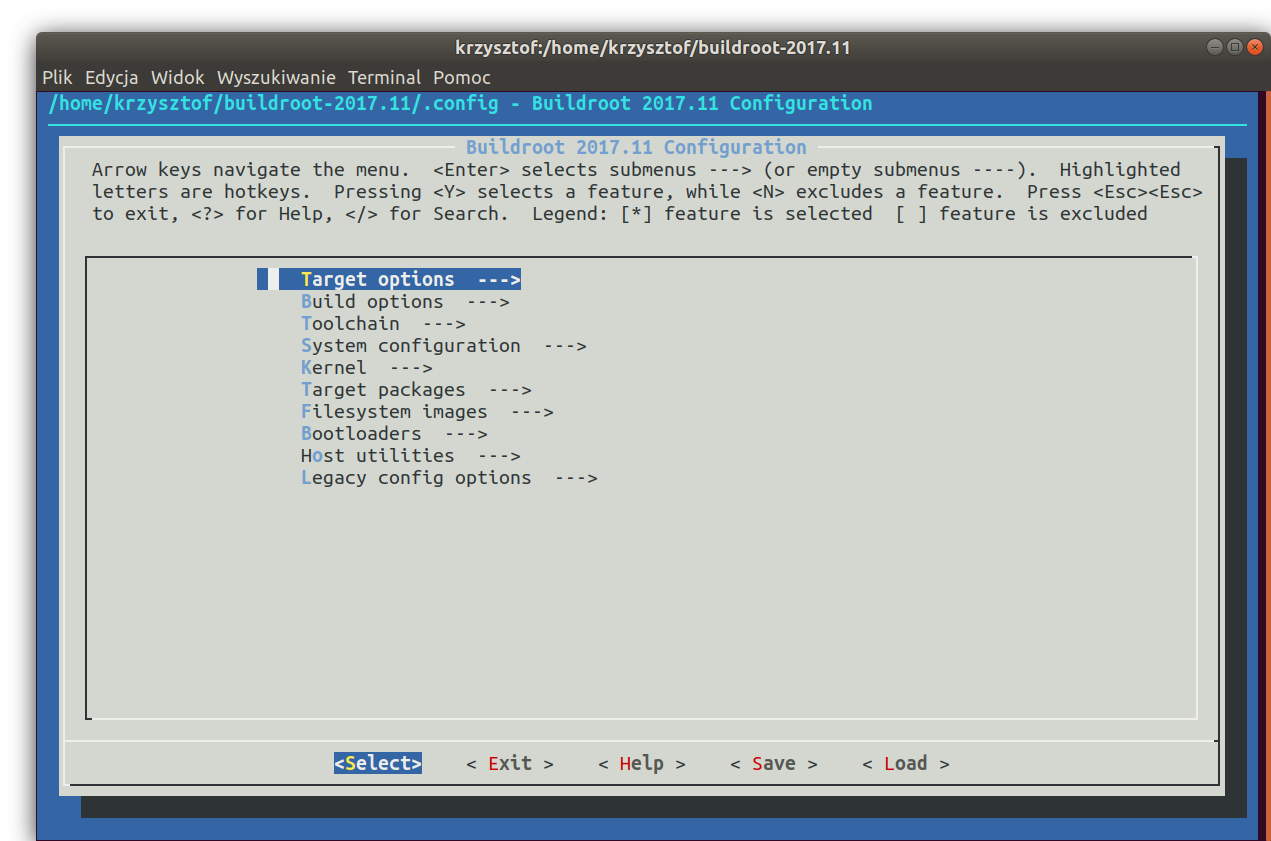
\includegraphics[width=13cm]{buildroot_menu}
	\caption{Widok głównego menu środowiska Buildroot} 
	\label{fig:brmenuconfig}
\end{figure}

\subsection{Toolchain}

Toolchain jest zestawem narzędzi programistycznych, pozwalających na wykonanie cross-kompilacji programu na maszynie o innej architekturze. Składa się z kompilatora, linkera oraz bibliotek danego języka programowania. W środowisku Buildroot użytkownik ma możliwosć wybrania, czy Toolchain ma być stworzony przez środowisko zgodnie z opcjami dotyczącymi architektury sprzętu docelowego. Alternatywą jest podanie zewnętrznego zestawu narzędzi \ang{Toolchain} i dołączenie do projektu.

\subsection{Dodawanie modułów jądra}

Dodawanie skompilowanych modułów jądra odbywa się za pomocą komendy \ang{modprobe}. Kod modułu wraz z plikami konfiguracyjnymi należy dodać podczas konfiguracji środowiska Buildroot. Na etapie dokonywania zmian w kodzie sterownika, Buildroot umożliwia cross-kompilację wybranego pakietu. Skompilowany moduł wysyłano za pomocą połączenia ssh.


\section{Komunikacja z Raspberry Pi}

Na etapie rozwoju oprogramowania, debugowania oraz testów potrzebna była komunikacja pomiędzy komputerem PC, a płytką Raspberry Pi. Platforma posiada kilka różnych możliwości komunikacji, jednak najbardziej niezawodnym i dającym pełną informację o stanie systemu był port UART. Aby móc obsłużyć konwerter USB-UART i komunikować się z Raspberry Pi na komputerze PC posłużono się programem minicom.

Komunikacja przez port Ethernet, bądź WiFi za pomocą klienta SSH (a ang. Secure Shell) pozwalała na komunikację z większą przepustowością, co było istotne podczas testów systemu pod kątem akwizycji danych. 

\section{Sterowniki urządzeń}
Do obsługi urządzeń dołączanych do systemu przy pomocy magistral SPI i 
I$^2$C potrzebne są odpowiednie sterowniki urządzeń. Można skorzystać z gotowych modułów udostępniających aplikacjom użytkownika dostęp do pamięci urządzeń takich jak np. \ang{spidev}\cite{spidev} i \ang{i2c-dev}\cite{i2cdev}. W celu zapewnienia wydajnej pracy programom o ścisłym reżimie czasowym w projekcie zastosowano moduł do jądra systemu operacyjnego umożliwiający obsługę przetwornika analogowo-cyfrowego.

\subsection{Sterownik przetwornika analogowo-cyfrowego}

Projekt zakładał napisanie kodu sterownika urządzenia umożliwiającego dostęp aplikacji do magistrali SPI w celu odebrania pomiaru napięcia analogowego z jednego z ośmiu kanałów przetwornika analogowo-cyfrowego MAX1202. Użytkownik powinien mieć możliwość ustawienia okresu próbkowania przetwornika
oraz wyzwolenia i przerwania pomiaru z poziomu aplikacji. 

Komunikacja sterownika z aplikacją jest zapewniona poprzez urządzenie znakowe kw\_adc.
Do wysyłania komend do urządzenia zastosowano funkcję ioctl(). Przed pomiarem użytkownik ustawia za pomocą ioctl z komendą ADC\_SET czas pomiędzy przerwaniami (pole adc\_sampling\_period w strukturze dev) co powoduje ustawienie okresu próbkowania przetwornika. 
W jednym transferze wysyłany jest 1 bajt komendy (pomiar z CH1 to 0x9f) i jednocześnie odbierane są 2 bajty danych pomiarowych. 

Aby zaimplementować funkcjonalność zmiany częstotliwości próbkowania z poziomu aplikacji. 
użyto struktury hr\_timer. Po skończeniu odliczania przez licznik uruchamiana jest funkcja obsługi przerwania, następuje przygotowanie odpowiednich struktur do transferu bajtów poprzez magistralę SPI. Ustawiane są parametry transmisji. Pomiar jest zlecany przez funkcję spi\_async asynchronicznie, więc proces nie jest blokowany. Gdy transfer jest zakończony uruchamiana jest funkcja complete(), gdzie dane pomiarowe są wpisywane do bufora cyklicznego. Z poziomu użytkownika dane są dostępne dzięki funkcji poll(), w której proces odczytu jest usypiany jeśli w buforze nie ma wystarczającej ilości danych do czytania. Po wpisaniu danych do bufora proces oczekujący na dane jest budzony w funkcji complete().


Istotnym podczas pisania sterownika był fakt, że dane są odbierane w funkcji obsługi przerwania. Determinowało to użycie funkcji asynchronicznej, bo funkcja spi\_sync\_transfer może być usypiana, więc nie możemy użyć jej w kontekście obsługi przerwania.
Dokonując niewielkich zmian w konfiguracji zawartej w kodzie sterownika możliwe jest obsłużenie innych układów posiadających interfejs SPI. Zweryfikowaniu i ewentualnej zmianie powinny być poddane pola struktury \ang{spi\_transfer} opisującej parametry transferu spi, które są opisane w dokumentacji jądra systemu operacyjnego Linux.\cite{spiKernel}.

\subsection{Protokół synchronizacji czasu}

Aby otrzymać dokładną informację o czasie pobrania próbki z przetwornika lub czujnika potrzebna jest synchronizacja czasu pomiędzy urządzeniami, którą można zapewnić dzięki protokołowi synchronizacji czasu takim jak na przykład NTP (z ang. Network Time Protocol).
Domyślnie w systemie Raspbian Jessie działa usługa \ang{systemd-timesyncd}, która działa na podstawie protokołu SNTP (z ang. Simple NTP) i jest dużo mniej rozbudowana. W przeciwieństwie do NTP to tylko klient, który pobiera i aktualizuje czas w systemie. W przypadku gdy chcemy skorzystać z serwera NTP, najlepiej jest tę usługę wyłączyć\cite{ntp}.

\subsection{Znacznik czasu}

System akwizycji danych wraz z zapisaną wartością próbki zapisuje czas zebrania próbki. Wykorzystano czas systemowy, który został wcześniej zsynchronizowany z serwerem NTP.
Początkowo w pierwszym podejściu do problemu zastosowano rozwiązanie w przestrzeni użytkownika, przy użyciu funkcji \ang{getMicrotime()}. Funkcja ta pozwala na zapisanie znacznika czasu w [$\mu$s] z racji na to, że jest wywoływana z programu w przestrzeni użytkownika, nie daje dużej dokładności. Nie da się jednoznacznie stwierdzić ile czasu minie pomiędzy zapisaniem wartości znacznika czasu i zebraniem próbki, ponieważ proces może być wywłaszczany.

Większą dokładność osiągnięto stosując licznik \ang{hrtimer} w kodzie modułu jądra, który pozwala na odmierzanie czasu w nanosekundach. Na zwiększoną dokładność tego rozwiązania ma wpływ fakt, iż znacznik czasu jest zapisywany w przestrzeni jądra i dopiero później przekazywany do aplikacji użytkownika.

Dokładna wartość znacznika czasu jest przechowywana w strukturze \ang{timespec}. Pobrano tą wartość dzięki funkcji getnstimeofday() zwracającej czas w nanosekundach i zapisano w zmiennej 64-bitowej. Znacznik czasu przekazywano do sterownika wraz z wartością próbki za pomocą bufora kołowego.


Tak zebrane dane mogą być wykorzystane w aplikacji z przestrzeni użytkownika na obliczenie znacznika czasu każdej próbki. To rozwiązanie pozwala osiągnąć większą dokładność i stałość częstotliwości próbkowania.


\section{Drzewo urządzeń}
W celu uruchomienia swojego modułu do jądra napisano nakładkę na drzewo urządzeń i skompilowaną dodano do odpowiedniego katalogu /boot/overlays, a następnie dopisano w pliku /boot/config.txt nazwę nakładki. Podane w nakładce parametry transmisji danych między urządzeniem podłączonym do magistrali, a płytką Raspberry Pi są ustalane przy załadowaniu modułu. 


\section{Aplikacje w przestrzeni użytkownika}

Programy użytkownika umożliwiają wyświetlenie danych zebranych przez niższą warstwę systemu. Wyniki pomiarów są zapisywane w plikach tekstowych i udostępniane sieciowo.

\subsection{Aplikacja wykorzystująca moduł \ang{spidev}}

W celu porównania wydajności i parametrów akwizycji danych różnych rozwiązań programowych napisano program wykorzystujący moduł \ang{spidev}. Moduł ten pozwala na odczyt danych doprowadzonych do magistrali SPI z poziomu aplikacji użytkownika. W rozdziale 5 przedstawiono wyniki testów i porównanie zmienności częstotliwości próbkowania. Aplikacja daje możliwość odczytu jednorazowego lub ciągłego z zadanym opóźnieniem. Opóźnienie jest ustalane za pomocą parametru \ang{delay\_usecs}, będącego polem struktury \ang{spi\_ioc\_transfer}. Komunikacja ze sterownikiem \ang{spidev} jest zapewniona za pomocą funkcji \ang{ioctl()} z komendą \ang{SPI\_IOC\_MESSAGE}. Komenda jest wywoływana w pętli głównej programu, a odebrane dane z przetwornika są zapisywane do bufora. Następnie pomiar jest zapisywany do pliku wraz ze znacznikiem czasu.

\subsection{Aplikacje wykorzystująca moduł \ang{i2cdev}}

W celu obsłużenia czujników podłączanych przez magistralę I$^2$C wykorzystano moduł \ang{i2cdev}. Moduł ten pozwala na odczyt danych doprowadzonych do magistrali SPI z poziomu aplikacji użytkownika. 

Przydatnym narzędziem przy korzystaniu z magistrali I$^2$C w Raspberry Pi jest pakiet \ang{i2c-tools}. Po zainstalowaniu pakietu, można skorzystać z komendy \ang{i2cdetect}, która wysyła zapytanie o adres urządzeń podłączonych do magistrali. W wyniku wyświetlana jest tablica urządzeń wraz z ich adresami jak przedstawiono na Rys. \ref{fig:i2cdetect}. Narzędzie umożliwia szybkie sprawdzenie, czy nie powstaje konflikt adresów pomiędzy urządzeniami dołączonymi do jednej magistrali oraz szybsze debugowanie błędów.

\begin{figure}[h]
	\centering
		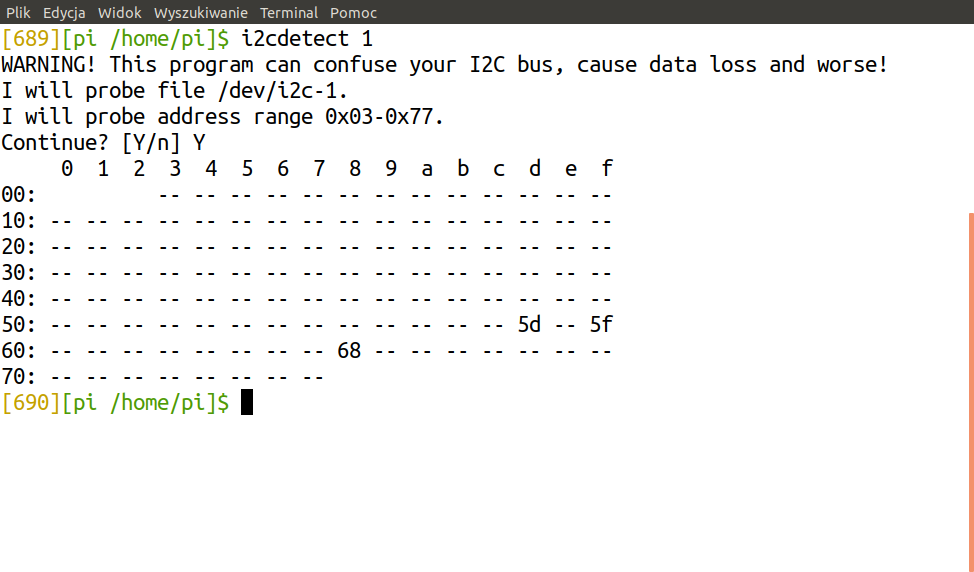
\includegraphics[width=13cm]{i2cdetect}
	\caption{Tablica adresów urządzeń podłączonych do magistrali I$^2$C} 
	\label{fig:i2cdetect}
\end{figure}


\subsection{Programy publikujące i subskrybujące dane przy pomocy protokołu MQTT}

Programy implementujące klienta i brokera MQTT napisano w języku Python w wersji 2 wykorzystując pakiet paho.mqtt.client, który udostępnia funkcje umożliwiające w łatwy sposób implementację aplikacji. 
Aplikacja publikująca publish.py wykonywana jest na Raspberry Pi i zawiera kod, który powoduje wysyłanie w pętli kolejno zebranych próbek. Publikacja zostaje nazwana tematem 
\ang{client.publish("test\_mqtt", file\_content[l]);)}.
W aplikacji klienta subscribe.py zawarty temat subskrybcji, który musi być zgodny z tematem zawartym w aplikacji publikującej dane\cite{paho.mqtt}
client.subscribe("test\_mqtt")

Program odpowiadający za odebranie danych zawiera informację na temat połączenia sieciowego: adres IP oraz numer portu.

\subsection{Aplikacja internetowa}

Aplikacja została napisana w języku php i html. Użytkownik jest w stanie uruchomić proces oraz go wyłączyć, korzystając z identyfikatora procesu zwracanego przez funkcję  \ang{shell\_exec}. Identyfikator uruchomionego procesu zapisywany jest w pliku pid.txt. Dane zebrane przez czujniki zapisywane są w pliku tekstowym w katalogu, z którego była wywołana aplikacja. W przypadku wywołania z aplikacji internetowej jest to katalog \ang{/var/www/html}. Parametry akwizycji danych mogę być ustawiane z poziomu aplikacji internetowej i zapisane do pliku konfiguracyjnego. Informacja o parametrach pomiarów jest wczytywana z pliku konfiguracyjnego przez program obsługujący dany czujnik. Po odebraniu próbki użytkownik jest w stanie podejrzeć aktualną wartość odczytaną z sensora uruchamiając aplikacją obsługującą protokół MQTT. 

